\documentclass[11pt,a4paper]{article}
\usepackage[T1]{fontenc}
\usepackage[ngerman]{babel}
\usepackage{amsmath}
\usepackage{parskip}
\usepackage{graphicx}
\usepackage{listings}

%opening
\author{Simon Cholewa}
\title{3. Excercises PDS}

\hyphenation{
	Mo-tor-ü-ber-wach-ung 
}


\begin{document}

\maketitle

\section{IDE Set Up}
\textit{Set Up your IDE or at least a good editor for Python with a Python mode/ support! (name + personal screenshot included)}

Abbildung \ref{fig:pycharm} auf zeigt einen Screenshot meiner PyCharm-Installation.

\begin{figure}[!htbp] 
	\centering
	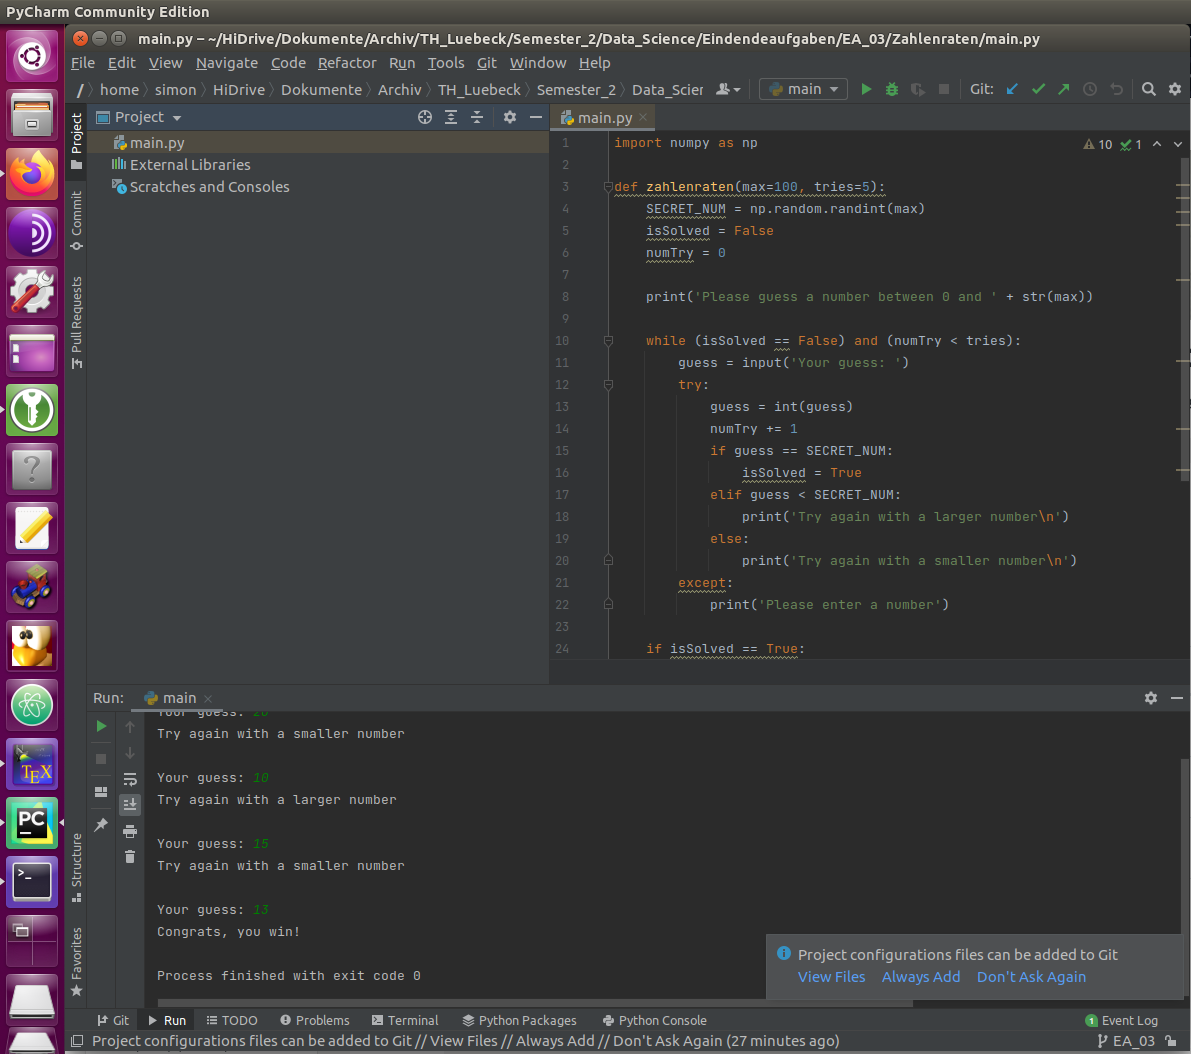
\includegraphics[width=1.0\linewidth]{images/PyCharm}
	\caption[PyCharm]{PyCharm 2021.1 installiert und konfiguriert.}
	\label{fig:pycharm}
\end{figure}


\section{Dive into Python}
\textit{Write a tiny game or everything else in Python to get fluent in Python. No fancy graphics needed. A tic-tac-toe on console is fine. If you already wrote Python code, send me the GitHub Link or a part of the code in the PDF with an explanation (I will Goole the code, so no copycat, please ;-)}

Hier habe ich wirklich ein klassisches Minimalbeispiel für ein Konsolenspiel in Python programmiert. Der Spieler hat eine bestimmte Anzahl an versuchen, eine Zufallszahl zu erraten. Als Hinweis erhält er die Information, ob die gesuchte Zahl größer oder kleiner als der Tipp ist. Siehe dazu auch Abbildung \ref{fig:pycharm} aus der vorherigen Aufgabe.

Umgesetzt ist das Spiel in einer Funktion \texttt{zahlenraten}, die im Hauptprogramm mit dem Parameter 50 aufgerufen wird (Z.~31), welcher den Standardwert von 100 für den Wertebereich ersetzt. Für die maximale Anzahl an Rateversuchen wird das Default von 5 (Z.~3) nicht geändert. Für die Berechnung der gesuchten Zahl wird nutzt Numpy genutzt (Z.~4).

\bigskip

\lstinputlisting[numbers=left, language=Python, frame=single, tabsize=2, basicstyle=\footnotesize, showstringspaces=false]{Zahlenraten/main.py}

In einer \texttt{while}-Schleife (Z.~10) werden so lange Zahlen von der Tastatur eingelesen, bis keine Versuche mehr verfügbar sind oder die gesuchte Zahl erraten wurde. Zum Einlesen der Tastatureingaben wird \texttt{input()} eigesetzt. Da hier auch Strings eingelesen werden können, wird versucht (Z.~12), die Eingabe in einen Integer umzuwandeln (Z.~13). Falls das fehlschlagen sollte, weil beispielsweise ein Buchstabe eingegeben wurde, wird der \texttt{except}-Teil ausgeführt. Der Zähler für die Versuche wird nicht inkrementiert.

\end{document}
